% A LaTeX template for EXECUTIVE SUMMARY of the MSc Thesis submissions to 
% Politecnico di Milano (PoliMi) - School of Industrial and Information Engineering
%
% S. Bonetti, A. Gruttadauria, G. Mescolini, A. Zingaro
% e-mail: template-tesi-ingind@polimi.it
%
% Last Revision: October 2021
%
% Copyright 2021 Politecnico di Milano, Italy. NC-BY

\documentclass[11pt,a4paper,twocolumn]{article}

%------------------------------------------------------------------------------
%	REQUIRED PACKAGES AND  CONFIGURATIONS
%------------------------------------------------------------------------------
% PACKAGES FOR TITLES
\usepackage{titlesec}
\usepackage{color}

% PACKAGES FOR LANGUAGE AND FONT
\usepackage[utf8]{inputenc}
\usepackage[english]{babel}
\usepackage[T1]{fontenc} % Font encoding

% PACKAGES FOR IMAGES
\usepackage{graphicx}
\graphicspath{{Images/}} % Path for images' folder
\usepackage{eso-pic} % For the background picture on the title page
\usepackage{subfig} % Numbered and caption subfigures using \subfloat
\usepackage{caption} % Coloured captions
\usepackage{transparent}

% STANDARD MATH PACKAGES
\usepackage{amsmath}
\usepackage{amsthm}
\usepackage{bm}
\usepackage[overload]{empheq}  % For braced-style systems of equations

% PACKAGES FOR TABLES
\usepackage{tabularx}
\usepackage{longtable} % tables that can span several pages
\usepackage{colortbl}

% PACKAGES FOR ALGORITHMS (PSEUDO-CODE)
\usepackage{algorithm}
\usepackage{algorithmic}

% PACKAGES FOR REFERENCES & BIBLIOGRAPHY
\usepackage[colorlinks=true,linkcolor=black,anchorcolor=black,citecolor=black,filecolor=black,menucolor=black,runcolor=black,urlcolor=black]{hyperref} % Adds clickable links at references
\usepackage{cleveref}
\usepackage[square, numbers, sort&compress]{natbib} % Square brackets, citing references with numbers, citations sorted by appearance in the text and compressed
\bibliographystyle{plain} % You may use a different style adapted to your field

% PACKAGES FOR THE APPENDIX
\usepackage{appendix}

% PACKAGES FOR ITEMIZE & ENUMERATES 
\usepackage{enumitem}

% OTHER PACKAGES
\usepackage{amsthm,thmtools,xcolor} % Coloured "Theorem"
\usepackage{comment} % Comment part of code
\usepackage{fancyhdr} % Fancy headers and footers
\usepackage{lipsum} % Insert dummy text
\usepackage{tcolorbox} % Create coloured boxes (e.g. the one for the key-words)
\usepackage{stfloats} % Correct position of the tables
\usepackage{comment} % To create block comments

%-------------------------------------------------------------------------
%	NEW COMMANDS DEFINED
%-------------------------------------------------------------------------
% EXAMPLES OF NEW COMMANDS -> here you see how to define new commands
\newcommand{\bea}{\begin{eqnarray}} % Shortcut for equation arrays
\newcommand{\eea}{\end{eqnarray}}
\newcommand{\e}[1]{\times 10^{#1}}  % Powers of 10 notation
\newcommand{\mathbbm}[1]{\text{\usefont{U}{bbm}{m}{n}#1}} % From mathbbm.sty
\newcommand{\pdev}[2]{\frac{\partial#1}{\partial#2}}
% NB: you can also override some existing commands with the keyword \renewcommand

%----------------------------------------------------------------------------
%	ADD YOUR PACKAGES (be careful of package interaction)
%----------------------------------------------------------------------------


%----------------------------------------------------------------------------
%	ADD YOUR DEFINITIONS AND COMMANDS (be careful of existing commands)
%----------------------------------------------------------------------------


% Do not change Configuration_files/config.tex file unless you really know what you are doing. 
% This file ends the configuration procedures (e.g. customizing commands, definition of new commands)
% Set the geometric layout of the document
\usepackage{geometry}
\geometry{
  top=3cm,
  left = 2.0cm,
  right = 2.0cm,
  bottom=2cm,
  headheight= 2cm,
  headsep= 0cm,
}
\raggedbottom 

\definecolor{WEBrown}{cmyk}{0.4,0.1,0,0.4}
\definecolor{WEBrown}{RGB}{148, 101, 76}

% Custom theorem environments
\declaretheoremstyle[
  headfont=\color{WEBrown}\normalfont\bfseries,
  bodyfont=\color{black}\normalfont\itshape,
]{colored}

\captionsetup[figure]{labelfont={color=WEBrown}} % Set colour of the captions
\captionsetup[table]{labelfont={color=WEBrown}} % Set colour of the captions
\captionsetup[algorithm]{labelfont={color=WEBrown}} % Set colour of the captions

\theoremstyle{colored}
\newtheorem{theorem}{Theorem}[section]
\newtheorem{proposition}{Proposition}[section]

% Enhances the features of the standard "table" and "tabular" environments.
\newcommand\T{\rule{0pt}{2.6ex}}
\newcommand\B{\rule[-1.2ex]{0pt}{0pt}}

% Algorithm description
\newcounter{algsubstate}
\renewcommand{\thealgsubstate}{\alph{algsubstate}}
\newenvironment{algsubstates}{
    \setcounter{algsubstate}{0}%
    \renewcommand{\STATE}{%
    \stepcounter{algsubstate}%
    \Statex {\small\thealgsubstate:}\space}
    }{}
    
% Custom theorem environment
\newcolumntype{L}[1]{>{\raggedright\let\newline\\\arraybackslash\hspace{0pt}}m{#1}}
\newcolumntype{C}[1]{>{\centering\let\newline\\\arraybackslash\hspace{0pt}}m{#1}}
\newcolumntype{R}[1]{>{\raggedleft\let\newline\\\arraybackslash\hspace{0pt}}m{#1}}

% Custom itemize environment
\setlist[itemize,1]{label=$\bullet$}
\setlist[itemize,2]{label=$\circ$}
\setlist[itemize,3]{label=$-$}
\setlist{nosep}

% Set separation of columns 
\setlength{\columnsep}{30pt}

% Create command for background pic
\newcommand\BackgroundPic{% Adding background picture
	\put(230,358){
		\parbox[b][\paperheight]{\paperwidth}{%
			\vfill
			\centering
			\transparent{0.4}
			
\includegraphics[width=0.5\paperwidth]{raggiera_polimi.eps}%
			\vfill
}}}

% Set indentation
\setlength\parindent{0pt}

% Custom title commands
\titleformat{\section}
{\color{WEBrown}\normalfont\Large\bfseries}
{\color{WEBrown}\thesection.}{1em}{}
\titlespacing*{\section}
{0pt}{2ex}{1ex}

\titleformat{\subsection}
{\color{WEBrown}\normalfont\large\bfseries}
{\color{WEBrown}\thesubsection.}{1em}{}
\titlespacing*{\subsection}
{0pt}{2ex}{1ex}

% Custom headers and footers
\pagestyle{fancy}
\fancyhf{}
      
\fancyfoot{}
\fancyfoot[C]{\thepage} % page
\renewcommand{\headrulewidth}{0mm} % headrule width
\renewcommand{\footrulewidth}{0mm} % footrule width

\makeatletter
\patchcmd{\headrule}{\hrule}{\color{black}\hrule}{}{} % headrule
\patchcmd{\footrule}{\hrule}{\color{black}\hrule}{}{} % footrule
\makeatother

% -> Create the header
\chead[C]{
\centering
\begin{tcolorbox}[arc=0pt, boxrule=0pt, colback=WEBrown!60, width=\textwidth, colupper=white]
    \textbf{Report} \hfill \textbf{\author}  
\end{tcolorbox}
}

% Insert here the info that will be displayed into your Title page 
% -> title of your work
\renewcommand{\title}{Experiment 2: PID Controller for the Fan Heater}
% -> author name and surname
\renewcommand{\author}{Gökhan Koçmarlı}
% -> MSc course
\newcommand{\course}{Introduction to Control Engineering}
% -> advisor name and surname
\newcommand{\advisor}{dr hab. inż. Paweł Dworak}
% IF AND ONLY IF you need to modify the co-supervisors you also have to modify the file Configuration_files/title_page.tex (ONLY where it is marked)
%\newcommand{\firstcoadvisor}{Name Surname} % insert if any otherwise comment
%\newcommand{\secondcoadvisor}{Name Surname} % insert if any otherwise comment
% -> academic year
\newcommand{\YEAR}{11-04-2022}

%-------------------------------------------------------------------------
%	BEGIN OF YOUR DOCUMENT
%-------------------------------------------------------------------------
\begin{document}

%-----------------------------------------------------------------------------
% TITLE PAGE
%-----------------------------------------------------------------------------
% Do not change Configuration_files/TitlePage.tex (Modify it IF AND ONLY IF you need to add or delete the Co-advisors)
% This file creates the Title Page of the document
% DO NOT REMOVE SPACES BETWEEN LINES!

\twocolumn[{\begin{@twocolumnfalse}

\AddToShipoutPicture*{\BackgroundPic}

\hspace{-0.2cm}
\includegraphics[width=0.6\textwidth]{Images/WydzialElectriczny.png}

\vspace{2mm}
\fontsize{0.3cm}{0.7cm}\selectfont \bfseries \textsc{\color{WEBrown} \course}\\

\vspace{-0.2cm}
\Large{\textbf{{\title}}}\\


\vspace{-0.2cm}
\fontsize{0.3cm}{0.5cm} \selectfont \bfseries Author: \textsc{\textbf{\author}}\\

\vspace{-0.4cm}
\fontsize{0.3cm}{0.5cm}\selectfont \bfseries Advisor: \textsc{\textbf{\advisor}}\\

% if only ONE co-advisor is present:
% \vspace{-0.4cm}
% \fontsize{0.3cm}{0.5cm}\selectfont \bfseries Co-advisor: \textsc{\textbf{\firstcoadvisor}}\\
% if more than one co-advisors are present:
%\vspace{-0.4cm}
%\fontsize{0.3cm}{0.5cm}\selectfont \bfseries Co-advisors: \textsc{\textbf{\firstcoadvisor}}\textsc{\textbf{\secondcoadvisor}}\\

\vspace{-0.4cm}
\fontsize{0.3cm}{0.5cm}\selectfont \bfseries Date: \textsc{\textbf{\YEAR}}

\small \normalfont

\vspace{11pt}

\centerline{\rule{1.0\textwidth}{0.4pt}}

\vspace{15pt}
\end{@twocolumnfalse}}]

\thispagestyle{plain} % In order to not show the header in the first page

%%%%%%%%%%%%%%%%%%%%%%%%%%%%%%
%%     LAB MAIN TEXT        %%
%%%%%%%%%%%%%%%%%%%%%%%%%%%%%%

% ===========================================================
% Introduction
% ===========================================================
\section{Introduction}
\label{sec:introduction}

This document is intended to be the second report of the laboratory homeworks. The objective of the homework is to understand how a real plant can be investigated, how to get output data into directly computer using I/Os and MATLAB, how to analyze the noisy output signal and construct a model, and how to tune a PID according to the model that will have been found.

% ===========================================================
% Experiments
% ===========================================================

\section{Experiments}
\label{sec:outputresponse4temp}

After connecting the necessary cables to record the data into MATLAB, we have created a Simulink model which has two inputs and two outputs. These two inputs are fan's motor power value and temperature value in terms of zero to ten. On the other hand, there are two outputs for motor speed and temperature values by sensors.

Within the pre-defined program, we could do experiments, and record the data of them as MAT files. All the data and graphs can be found on the link given end of the document.

One may see from the Table \ref{table:experimentsParameters}, the parameters (inputs) of the plant has no meanings in the value level. I mean, it is not important that "What does 4 actually represents?". In the control engineering perspective, the important thing is to have a change in parameter, and see the response of that given change.

One can see the oscillator graphs from the Figures \ref{fig:exp1OutputGraph}, \ref{fig:exp2OutputGraph}, \ref{fig:exp3OutputGraph}, and \ref{fig:exp4OutputGraph}.

\begin{table}[H]
    \centering 
    \begin{tabular}{|p{3em} c c |}
    \hline
    \rowcolor{WEBrown!40}
     & \textbf{Motor Input} & \textbf{Temperature Input} \T\B \\
    \hline \hline
    \textbf{Exp1} & 4 & from 5 to 3 \T\B \\
    \textbf{Exp2} & 4 & from 6 to 5 \T\B \\
    \textbf{Exp3} & 6 & from 3 to 6 \T\B \\
    \textbf{Exp4} & 6 & from 6 to 5 \T\B \\
    \hline
    \end{tabular}
    \\[10pt]
    \caption{Experiments that we have done to find model of the plant.}
    \label{table:experimentsParameters}
\end{table}

\begin{figure}[H]
    \centering
    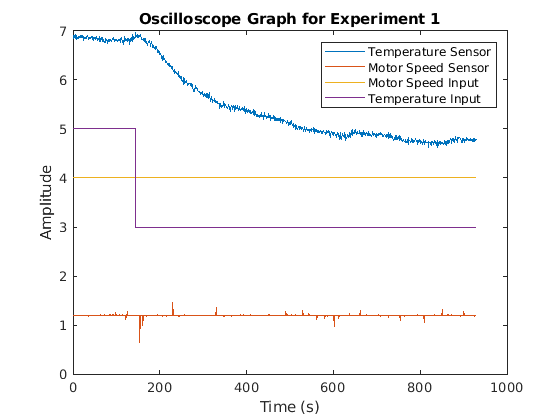
\includegraphics[width=0.5\textwidth]{Graphs/Exp1Osc.png}
    \caption{Oscillator Graph for the Experiment 1}
    \label{fig:exp1OutputGraph}
\end{figure}
\begin{figure}[H]
    \centering
    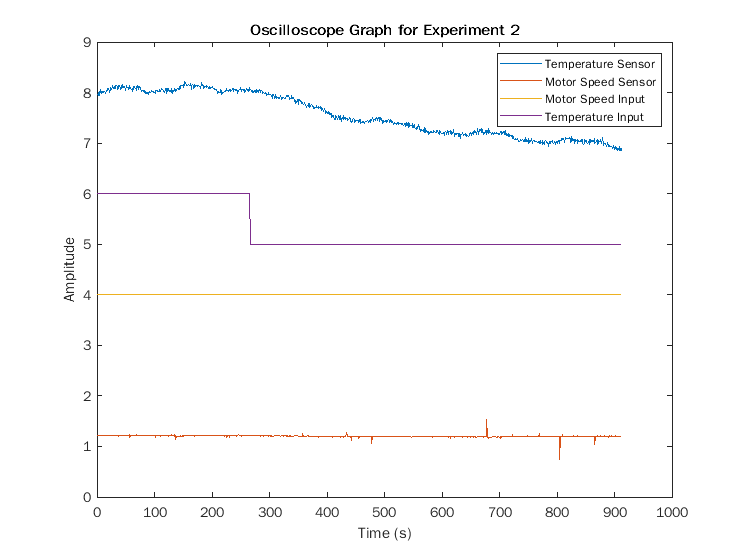
\includegraphics[width=0.5\textwidth]{Graphs/Exp2Osc.png}
    \caption{Oscillator Graph for the Experiment 2}
    \label{fig:exp2OutputGraph}
\end{figure}
\begin{figure}[H]
    \centering
    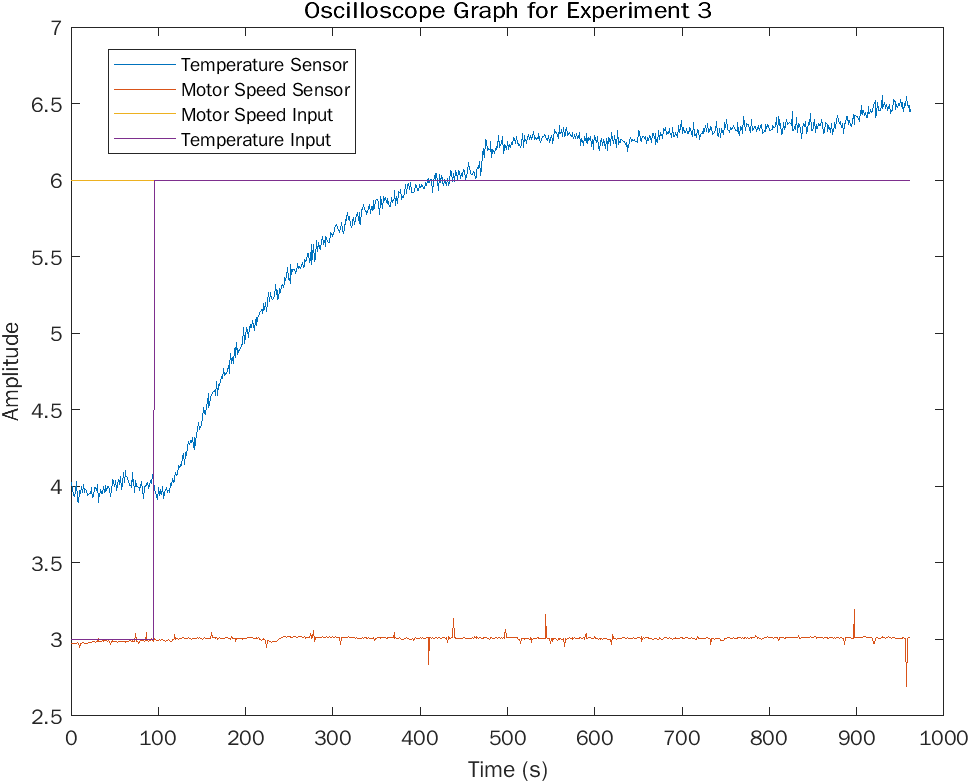
\includegraphics[width=0.5\textwidth]{Graphs/Exp3Osc.png}
    \caption{Oscillator Graph for the Experiment 3}
    \label{fig:exp3OutputGraph}
\end{figure}
\begin{figure}[H]
    \centering
    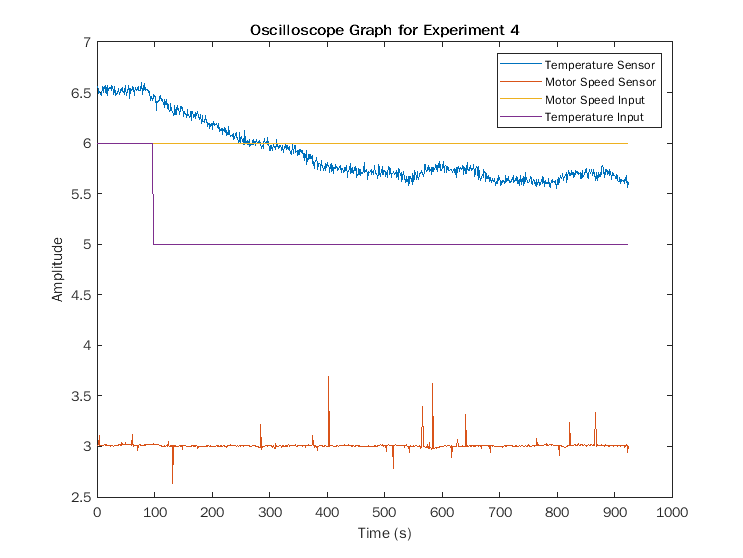
\includegraphics[width=0.46\textwidth]{Graphs/Exp4Osc.png}
    \caption{Oscillator Graph for the Experiment 4}
    \label{fig:exp4OutputGraph}
\end{figure}

On the next section, we're going to create different models for each experiment. In non-liner models, the professor suggests that, it is reasonable to have more than one model within its range of parameters.

% ===========================================================
% Modelling with System Identification Tool
% ===========================================================

\section{Modelling with System Identification Tool}
\label{sec:modellingthestepresponse}

To model a step response of a plant, we can use the tool Identification Tool from System Identification Toolbox in MATLAB. In this document, we're going to use it since its algorithms much more effective comparing to our sense -- and knowledge. In order to open the tool, one can call the command \textit{systemIdentification} on MATLAB Command View.

\begin{figure}[H]
    \centering
    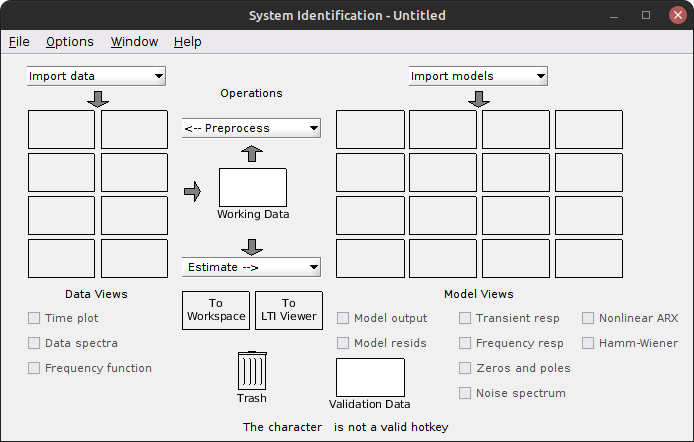
\includegraphics[width=0.48\textwidth]{Graphs/SystemIdentificationToolApp.png}
    \caption{GUI of the System Identification App on MATLAB}
\end{figure}

We will introduce you to how to perform a modelling operation for our first experiment, however, one can do every step detailed if they want to achieve the models for other experiments.

\begin{enumerate}
    \item Since our data is time-based, we will choose \textit{Time Domain Data} from \textit{Import Data} combobox.
    \item In the recently shown window, it asks us \textit{Workspace Variables} and \textit{Data Information}. In the Workspace Variables section, the input variable is the data that we fed into the plant -- for our case, it is the step function that goes from 5 to 3. On the other hand, the output variable is the sensors' data that we've collected. the Data Information section ask you details about your data. For example, data-name can be anything you want, however, sample time is crucial for our model. In the experiment, we have used a delay of 0.2 seconds between the experiments.
    \item One can verify the data with clicking \textit{Time plot} checkbox on the window.
    \item After the process of inputting the data, we are ready to process it. In the \textit{Estimate ->} combobox, one should select \textit{Process Models} in order to find a plant model.
    \item The new window, that is opened, is a very valuable tool for us. Selecting the transfer function's details, and clicking the Estimate button, gives us the model that we want. Since we want best results, I'll try all the combinations of transfer function, and look into their achievement percentage.
\end{enumerate}

\subsection{Comparison of Models}
I had done several estimation types for the first experiment's data. These can be seen in the unordered list below, and also the similarity of the model according to real data can be seen as a percentage.

\begin{itemize}
    \item P1: One Pole -- 87.88\%
    \item P2: Two Pole -- 81.86\%
    \item P1Z: One Pole, One Zero -- 88.68\%
    \item P2Z: Two Pole, One Zero -- 88.45\%
    \item P1D: One Pole, One Delay -- 87.32\%
    \item P2D: Two Pole, One Delay -- 87.49\%
    \item P1I: One Pole, One Integrator -- -116.9\%
    \item P2I: Two Pole, One Integrator -- -1572\%
    \item P1DZ: One Pole, One Delay, One Zero -- 88.26\%
    \item P2DZ: Two Pole, One Delay, One Zero -- 73.74\%
    \item P1IZ: One Pole, One Integrator, One Zero -- -2687\%
    \item P2IZ: Two Pole, One Integrator, One Zero -- 64.87\%
    \item P1DI: One Pole, One Delay, One Integrator -- -102.4\%
    \item P2DI: Two Pole, One Delay, One Integrator -- 75.64\%
    \item P1DIZ: One Pole, One Delay, One Integrator, One Zero -- -98.76\%
    \item P2DIZ: Two Pole, One Delay, One Integrator, One Zero -- 60.5\%
\end{itemize}

One can see that the most three similarity is P1Z, P2Z, and P1DZ.

\begin{figure}[H]
    \centering
    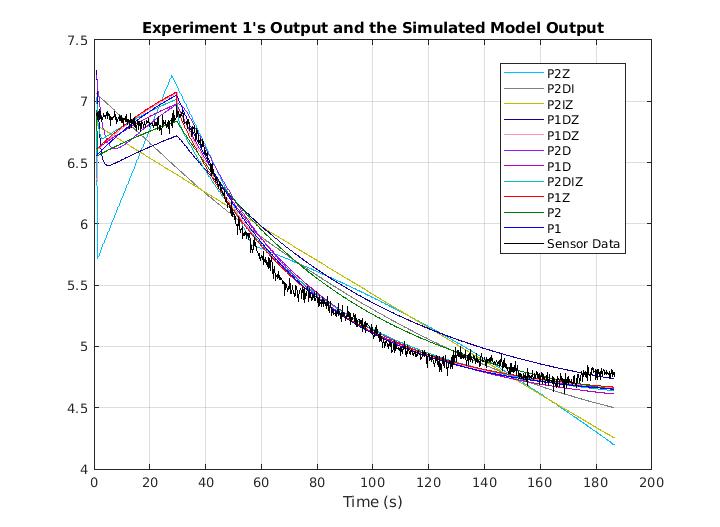
\includegraphics[width=0.5\textwidth]{Graphs/Exp1Output-SimulatedModel.png}
    \caption{Estimated Model's Simulations vs Real Data for Experiment 1}
\end{figure}

Since we found an achievement nearly $\approx 88\%$, you might think that we're going to use the model of P1Z which is described in \eqref{eq:EX1-BestModel}. One should note that the best model is not the model is very similar to our data, but the model which is reasonable for our plant. All of our experiment will tell you the best model is with zeros, maybe, however, having a zero will create a pike in the reverse direction of our desire in the first stages of the process. It is not reasonable.

\begin{equation}
    G(s) = 1.5271 \cdot \frac{1 + 2.2184s}{1 + 47.506s}
    \label{eq:EX1-BestModel}
\end{equation}

Also, it is not enough if we found a model of P1 or P2. We need a delay coefficient due to division of zero error in the tuning operation of PIDs.

However, we can use P1 model for our controller, since it is one of the basic ones in the list. That model has an accuracy of 87.88\% which is nearly 88\% as the best model. You can see the mathematical model inside the Eq. \eqref{eq:EX1-Model}. Notice that, it doesn't include any delay at all.

\begin{equation}
    G(s) = \frac{1.5232}{1 + 45.891s}
    \label{eq:EX1-Model}
\end{equation}

% ===========================================================
% Modelling Trail and Error
% ===========================================================

\section{Modelling by Trial \& Error}
\label{sec:modeltrialerror}
As you can see the models that we have found for Experiment 1, none of the models are comfortable for us to create a controller for the plant. In such times, we can use the trail-and-error approach that is trying to guess the model by doing experiments on the signal response with Simulink.

Firstly, we add a transfer function with a transport delay into our Simulink design. One can give them any parameter they want. After, we have to check for the experimental output graph and our model graph for differences. One should consider the list above.

\begin{itemize}
    \item If our model starts in different position, we should add a constant value.
    \item If our model ends in different position, we should change the gain parameter.
    \item If our model starts to change in different time, we should change the delay coefficient.
    \item If our model's slope is not looking like the real data, we should change the coefficient of $s$ in the denominator.
\end{itemize}

% ===========================================================
% Other Experiments
% ===========================================================

\section{Other Experiments}
\label{sec:otherexperiments}
Let's make the same steps to the other experiments and find their best model. For each experiment, I'll introduce the best three model, and the graph for all the models and the real data. Also, you're going to see the best model in terms of mathematical expression with its accuracy rate.

After this section, we're going to discuss how should we combine the models, or should we combine them in the first hand. All the data, and the plots given on the website that you can find in the link end of the document.

This is a problem when we want to create a controller. Because nearly all methods includes delay constant on the denominator part in a division. We should add arbitrary delay if we have a non-delayed model.

\begin{figure}[H]
    \centering
    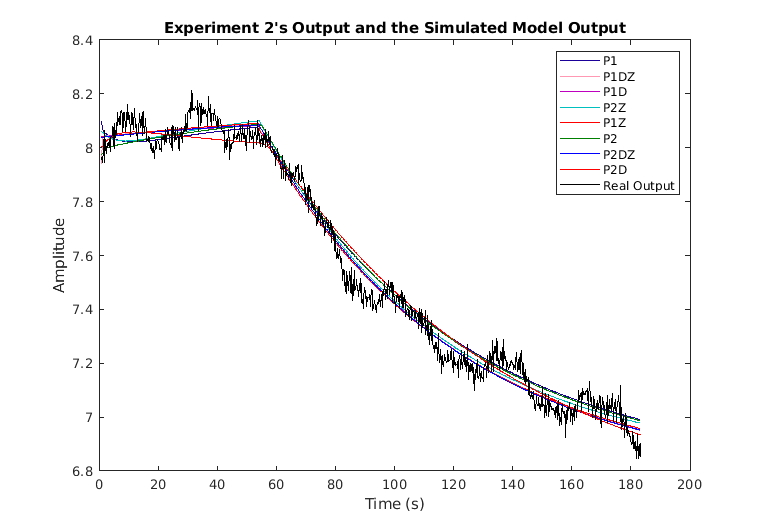
\includegraphics[width=0.5\textwidth]{Graphs/Exp2Output-SimulatedModel.png}
    \caption{Estimated Model's Simulations vs Real Data for Experiment 2}
\end{figure}

% ====== Second Experiment ====== 

For the second experiment, P1DZ, PIZ, and P1 are the best results we can find. The most accurate result is P1DZ, and the result is 87.32\%. One can see the model in the \eqref{eq:EX2-BestModel}. However, it is not an ideal model for our plant since it has zeros.

\begin{equation}
    G(s) = 1.3542 \cdot \frac{1+1.0128s}{1+66.063} \cdot e^{-0.2s}
    \label{eq:EX2-BestModel}
\end{equation}

The model can be used has the accuracy of 87.24\%, and one can see the model in Eq. \eqref{eq:EX2-Model}. Due to lack of delay, it will make us some problems to create a controller.

\begin{equation}
    G(s) = \frac{1.3536}{1+65.559}
    \label{eq:EX2-Model}
\end{equation}

% ====== Third Experiment ====== 

\begin{figure}[H]
    \centering
    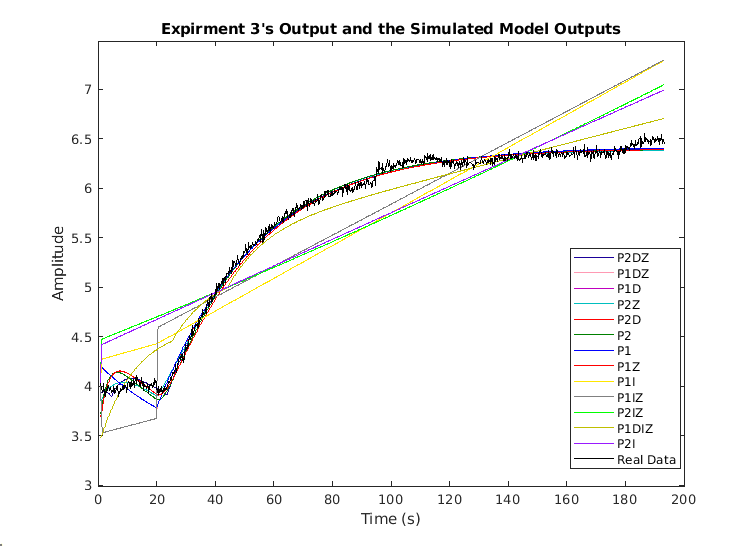
\includegraphics[width=0.46\textwidth]{Models/Exp3Output-SimulatedModel.png}
    \caption{Estimated Model's Simulations vs Real Data for Experiment 3}
\end{figure}

For the third experiment, P2DZ, P2Z, and P2 are the best results we can find. The most accurate result is P2DZ, and the result is 94.11\%. One can see the model in the \eqref{eq:EX3-BestModel}.

\begin{equation}
    G(s) = \frac{1.0687 \cdot (1+6.215s)}{(1+33.564s)(1+5.5575s)} \cdot e^{-3.5448s}
    \label{eq:EX3-BestModel}
\end{equation}

Again, the model doesn't respond to our needs. We should consider another model which is P1D with 92.69\% accuracy. You can see the model in Eq. \eqref{eq:EX3-Model}. We'll use it in our controller.

\begin{equation}
    G(s) = \frac{1.0708}{1+34.536s} \cdot e^{-0.0124s}
    \label{eq:EX3-Model}
\end{equation}

% ====== Fifth Experiment ====== 

\begin{figure}[H]
    \centering
    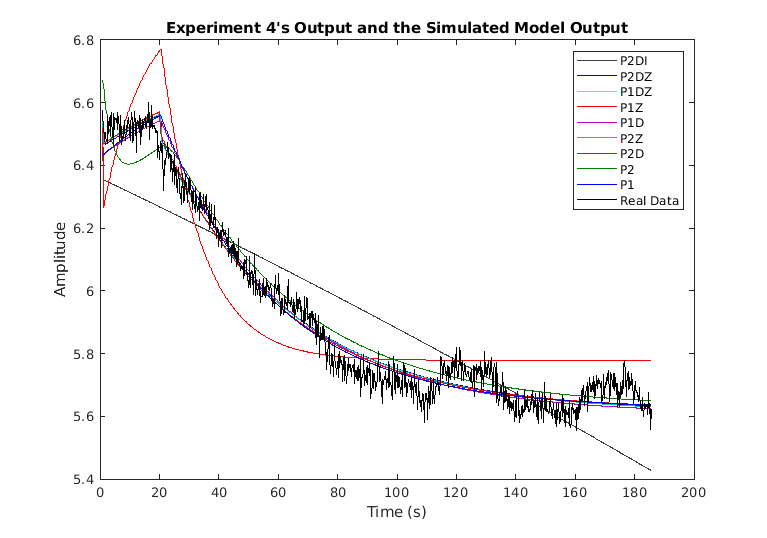
\includegraphics[width=0.50\textwidth]{Models/Exp4Output-SimulatedModel.png}
    \caption{Estimated Model's Simulations vs Real Data for Experiment 4}
\end{figure}

For the fourth experiment, P1Z, P1DZ, and P2Z are the best results we can find. The most accurate result is P1Z, and the result is 83.28\%. One can see the model in the \eqref{eq:EX4-BestModel}.

\begin{equation}
    G(s) = 1.1241 \cdot \frac{1+2.5994s}{1+40.751s}
    \label{eq:EX4-BestModel}
\end{equation}

Also, the model we're going to use will be P2D that has 82.53\% accuracy as the best model. You can find its function in Eq. \eqref{eq:EX4-Model}.

\begin{equation}
    G(s) = \frac{1.1556}{(1+13.684s)(1+0.0042803)} \cdot e^{-0.1844}
    \label{eq:EX4-Model}
\end{equation}

\subsection{Combining the Models}
Since our experiments are in different settings, which means in different times and different initial conditions, we cannot merge them into one model with \textit{merge()} function in MATLAB. As I asked our professor, dr. hab. Pawel Dworak, he told me that "We should create 4 different models, but you always have to specify (working point - for which motor speed (or pressure) and temperature they are valid). It's normal for nonlinear plants, and we have to deal with that in everyday practices". From the lines, we understand that creating a model for each condition is not-realistic, and will be very hard for us in this point of learning control engineering.

Therefore, we're going to only choose one model from our set of models to implement a PID controller for it. The model will be from Experiment 3 because of it has includes delay coefficient which is necessary for creating a controller.

\section{Controller Tuning}
\label{sec:controllertunning}
In this section, we're going to construct a PID controller for our model in the Eq. \eqref{eq:EX4-Model}. Since a machine can only have one controller, we can only use one model for a controller. Finding parameters of PID controller can be done with some formulas which can be found in the book "Handbook of PI and PID Controller Tuning Rules" by Aidan O'Dwyer. We're also going to represent them in here.

It is a SOSPD process model. So that, we can use the rules of that teacher give us, that is published on 1935.

\subsection{Calculation of Coefficients}

So we can find the $K_c$.
\begin{equation}
    K_c = \frac{0.95 T_m}{k_0 \tau_m}
\end{equation}
\begin{equation*}
    K_c = \frac{0.95 \cdot 34.536}{1.0708 \cdot 0.0124}
\end{equation*}
\begin{equation*}
    K_c \approx 2470.96
\end{equation*}

Time to find $T_i$ now.
\begin{equation}
    T_i = 2.4 \cdot \tau_m
\end{equation}
\begin{equation*}
    T_i = 2.4 \cdot 0.0124 = 0.02976
\end{equation*}

At last, let's find the $K_d$ parameter of PID controller.
\begin{equation}
    T_d = 0.4 \cdot \tau_m
\end{equation}
\begin{equation*}
    T_d = 0.4 \cdot = 0.00496
\end{equation*}

\subsubsection{Simulation of PID Controller}
Our controller will have the formula in Eq. \eqref{eq:PID-First}.
\begin{equation}
    C(s) = 2470.96 \left(1 + \frac{1}{0.02976s} + 0.00496s\right)
    \label{eq:PID-First}
\end{equation}

However, I found that the simulation is totally wrong due to the parameters of controller. If I use the \textit{pidTuner} in MATLAB, it gives me the parameters of Eq. \eqref{eq:ControllerModel}.

\begin{equation}
    K_c = 1.338\ \ T_i = 0.07012\ \ T_d = 0
    \label{eq:ControllerModel}
\end{equation}

You can find the results in Figures \ref{fig:SimResult1} and \ref{fig:SimResult2}.

\begin{figure}[H]
    \centering
    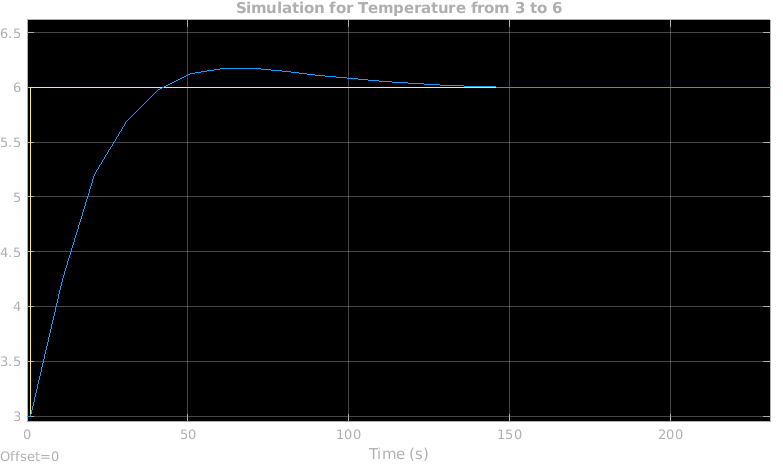
\includegraphics[width=0.5\textwidth]{Graphs/temp3to6.png}
    \caption{Temperature Input from 3 to 6}
    \label{fig:SimResult1}
\end{figure}
\begin{figure}[H]
    \centering
    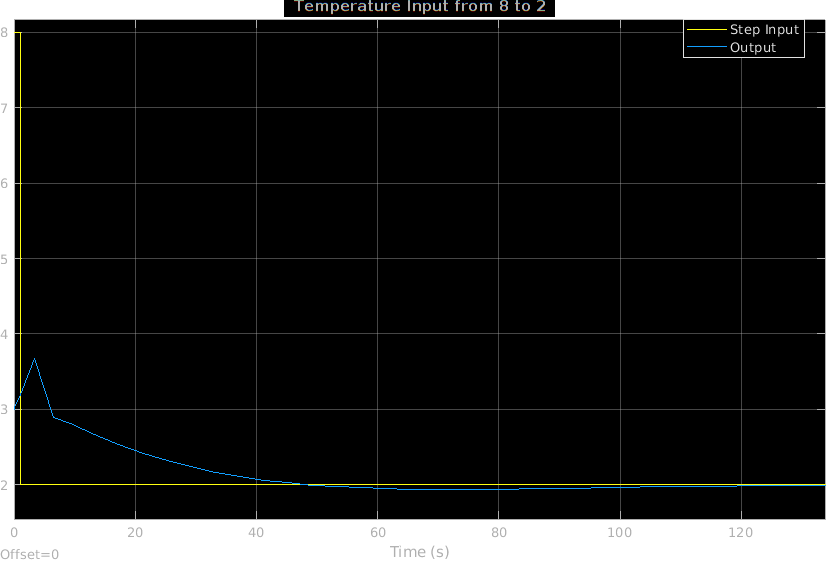
\includegraphics[width=0.5\textwidth]{Graphs/temp8to2.png}
    \caption{Temperature Input from 8 to 2}
    \label{fig:SimResult2}
\end{figure}

% ===========================================================
% Conclusions
% ===========================================================
\section{Conclusions}
\begin{itemize}
    \item Model is an approximation, don't make it too accurate.
    \item The most accurate model for a given dataset of a plant doesn't mean that is the best model for description of the plant. Before calculating our process models in any environment, we have to think about the way of working of our plant, and --not exactly, but at least-- think about its model.
    \item Zeros in the models creates an opposite direction starting according to our desire, which is non-wanted property for our solution. Some plants may need it.
    \item Real-life plants mostly are non-linear objects. It means that creating a model, and a controller from that model, doesn't give us a controller for every condition in the world. In fact, it will be a controller of a minuscule of all conditions. In the industrial level, most of the time environment is the same, therefore they can use PID controllers most of the time.
    \item For creating a model for changing states of environment, one can use adaptive control techniques.
    \item System Identification Toolbox gives us the models that we want easily, and very accuratly.
\end{itemize}

The reader should note all the files and the schemes can be found online at \url{https://dar.vin/Intro2ContrEng-LabOne-HeaterPID}.
% ===========================================================
% References
% ===========================================================
\section{References}
\begin{enumerate}
    \item Laboratory Document of First Experiment, dr. hab. Pawel Dworak, 2022
    \item Handbook of PI and PID Controller Tunning Rules, Aidan O'Dwyer, Imperial College Press, 2nd Edition
\end{enumerate}


\end{document}